\documentclass[1p]{elsarticle_modified}
%\bibliographystyle{elsarticle-num}

%\usepackage[colorlinks]{hyperref}
%\usepackage{abbrmath_seonhwa} %\Abb, \Ascr, \Acal ,\Abf, \Afrak
\usepackage{amsfonts}
\usepackage{amssymb}
\usepackage{amsmath}
\usepackage{amsthm}
\usepackage{scalefnt}
\usepackage{amsbsy}
\usepackage{kotex}
\usepackage{caption}
\usepackage{subfig}
\usepackage{color}
\usepackage{graphicx}
\usepackage{xcolor} %% white, black, red, green, blue, cyan, magenta, yellow
\usepackage{float}
\usepackage{setspace}
\usepackage{hyperref}

\usepackage{tikz}
\usetikzlibrary{arrows}

\usepackage{multirow}
\usepackage{array} % fixed length table
\usepackage{hhline}

%%%%%%%%%%%%%%%%%%%%%
\makeatletter
\renewcommand*\env@matrix[1][\arraystretch]{%
	\edef\arraystretch{#1}%
	\hskip -\arraycolsep
	\let\@ifnextchar\new@ifnextchar
	\array{*\c@MaxMatrixCols c}}
\makeatother %https://tex.stackexchange.com/questions/14071/how-can-i-increase-the-line-spacing-in-a-matrix
%%%%%%%%%%%%%%%

\usepackage[normalem]{ulem}

\newcommand{\msout}[1]{\ifmmode\text{\sout{\ensuremath{#1}}}\else\sout{#1}\fi}
%SOURCE: \msout is \stkout macro in https://tex.stackexchange.com/questions/20609/strikeout-in-math-mode

\newcommand{\cancel}[1]{
	\ifmmode
	{\color{red}\msout{#1}}
	\else
	{\color{red}\sout{#1}}
	\fi
}

\newcommand{\add}[1]{
	{\color{blue}\uwave{#1}}
}

\newcommand{\replace}[2]{
	\ifmmode
	{\color{red}\msout{#1}}{\color{blue}\uwave{#2}}
	\else
	{\color{red}\sout{#1}}{\color{blue}\uwave{#2}}
	\fi
}

\newcommand{\Sol}{\mathcal{S}} %segment
\newcommand{\D}{D} %diagram
\newcommand{\A}{\mathcal{A}} %arc


%%%%%%%%%%%%%%%%%%%%%%%%%%%%%5 test

\def\sl{\operatorname{\textup{SL}}(2,\Cbb)}
\def\psl{\operatorname{\textup{PSL}}(2,\Cbb)}
\def\quan{\mkern 1mu \triangleright \mkern 1mu}

\theoremstyle{definition}
\newtheorem{thm}{Theorem}[section]
\newtheorem{prop}[thm]{Proposition}
\newtheorem{lem}[thm]{Lemma}
\newtheorem{ques}[thm]{Question}
\newtheorem{cor}[thm]{Corollary}
\newtheorem{defn}[thm]{Definition}
\newtheorem{exam}[thm]{Example}
\newtheorem{rmk}[thm]{Remark}
\newtheorem{alg}[thm]{Algorithm}

\newcommand{\I}{\sqrt{-1}}
\begin{document}

%\begin{frontmatter}
%
%\title{Boundary parabolic representations of knots up to 8 crossings}
%
%%% Group authors per affiliation:
%\author{Yunhi Cho} 
%\address{Department of Mathematics, University of Seoul, Seoul, Korea}
%\ead{yhcho@uos.ac.kr}
%
%
%\author{Seonhwa Kim} %\fnref{s_kim}}
%\address{Center for Geometry and Physics, Institute for Basic Science, Pohang, 37673, Korea}
%\ead{ryeona17@ibs.re.kr}
%
%\author{Hyuk Kim}
%\address{Department of Mathematical Sciences, Seoul National University, Seoul 08826, Korea}
%\ead{hyukkim@snu.ac.kr}
%
%\author{Seokbeom Yoon}
%\address{Department of Mathematical Sciences, Seoul National University, Seoul, 08826,  Korea}
%\ead{sbyoon15@snu.ac.kr}
%
%\begin{abstract}
%We find all boundary parabolic representation of knots up to 8 crossings.
%
%\end{abstract}
%\begin{keyword}
%    \MSC[2010] 57M25 
%\end{keyword}
%
%\end{frontmatter}

%\linenumbers
%\tableofcontents
%
\newcommand\colored[1]{\textcolor{white}{\rule[-0.35ex]{0.8em}{1.4ex}}\kern-0.8em\color{red} #1}%
%\newcommand\colored[1]{\textcolor{white}{ #1}\kern-2.17ex	\textcolor{white}{ #1}\kern-1.81ex	\textcolor{white}{ #1}\kern-2.15ex\color{red}#1	}

{\Large $\underline{12n_{0381}~(K12n_{0381})}$}

\setlength{\tabcolsep}{10pt}
\renewcommand{\arraystretch}{1.6}
\vspace{1cm}\begin{tabular}{m{100pt}>{\centering\arraybackslash}m{274pt}}
\multirow{5}{120pt}{
	\centering
	\includegraphics[width=112pt]{../../../GIT/diagram.site/Diagrams/png/2470_12n_0381.png}\\
\ \ \ A knot diagram\footnotemark}&
\allowdisplaybreaks
\textbf{Linearized knot diagam} \\
\cline{2-2}
 &
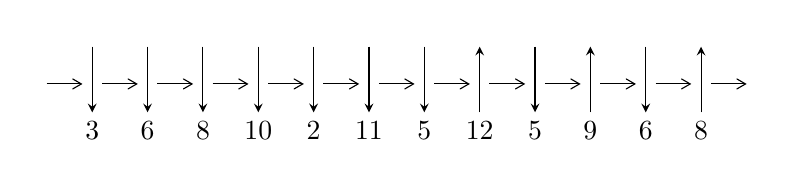
\begin{tikzpicture}[x=20pt, y=17pt]
	% nodes
	\node (C0) at (0, 0) {};
	\node (C1) at (1, 0) {};
	\node (C1U) at (1, +1) {};
	\node (C1D) at (1, -1) {3};

	\node (C2) at (2, 0) {};
	\node (C2U) at (2, +1) {};
	\node (C2D) at (2, -1) {6};

	\node (C3) at (3, 0) {};
	\node (C3U) at (3, +1) {};
	\node (C3D) at (3, -1) {8};

	\node (C4) at (4, 0) {};
	\node (C4U) at (4, +1) {};
	\node (C4D) at (4, -1) {10};

	\node (C5) at (5, 0) {};
	\node (C5U) at (5, +1) {};
	\node (C5D) at (5, -1) {2};

	\node (C6) at (6, 0) {};
	\node (C6U) at (6, +1) {};
	\node (C6D) at (6, -1) {11};

	\node (C7) at (7, 0) {};
	\node (C7U) at (7, +1) {};
	\node (C7D) at (7, -1) {5};

	\node (C8) at (8, 0) {};
	\node (C8U) at (8, +1) {};
	\node (C8D) at (8, -1) {12};

	\node (C9) at (9, 0) {};
	\node (C9U) at (9, +1) {};
	\node (C9D) at (9, -1) {5};

	\node (C10) at (10, 0) {};
	\node (C10U) at (10, +1) {};
	\node (C10D) at (10, -1) {9};

	\node (C11) at (11, 0) {};
	\node (C11U) at (11, +1) {};
	\node (C11D) at (11, -1) {6};

	\node (C12) at (12, 0) {};
	\node (C12U) at (12, +1) {};
	\node (C12D) at (12, -1) {8};
	\node (C13) at (13, 0) {};

	% arrows
	\draw[->,>={angle 60}]
	(C0) edge (C1) (C1) edge (C2) (C2) edge (C3) (C3) edge (C4) (C4) edge (C5) (C5) edge (C6) (C6) edge (C7) (C7) edge (C8) (C8) edge (C9) (C9) edge (C10) (C10) edge (C11) (C11) edge (C12) (C12) edge (C13) ;	\draw[->,>=stealth]
	(C1U) edge (C1D) (C2U) edge (C2D) (C3U) edge (C3D) (C4U) edge (C4D) (C5U) edge (C5D) (C6U) edge (C6D) (C7U) edge (C7D) (C8D) edge (C8U) (C9U) edge (C9D) (C10D) edge (C10U) (C11U) edge (C11D) (C12D) edge (C12U) ;
	\end{tikzpicture} \\
\hhline{~~} \\& 
\textbf{Solving Sequence} \\ \cline{2-2} 
 &
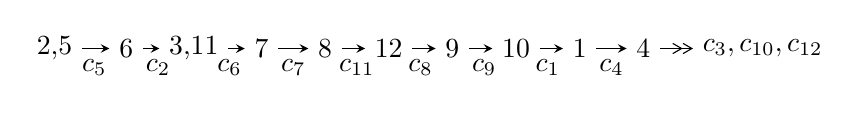
\begin{tikzpicture}[x=23pt, y=7pt]
	% node
	\node (A0) at (-1/8, 0) {2,5};
	\node (A1) at (1, 0) {6};
	\node (A2) at (33/16, 0) {3,11};
	\node (A3) at (25/8, 0) {7};
	\node (A4) at (33/8, 0) {8};
	\node (A5) at (41/8, 0) {12};
	\node (A6) at (49/8, 0) {9};
	\node (A7) at (57/8, 0) {10};
	\node (A8) at (65/8, 0) {1};
	\node (A9) at (73/8, 0) {4};
	\node (C1) at (1/2, -1) {$c_{5}$};
	\node (C2) at (3/2, -1) {$c_{2}$};
	\node (C3) at (21/8, -1) {$c_{6}$};
	\node (C4) at (29/8, -1) {$c_{7}$};
	\node (C5) at (37/8, -1) {$c_{11}$};
	\node (C6) at (45/8, -1) {$c_{8}$};
	\node (C7) at (53/8, -1) {$c_{9}$};
	\node (C8) at (61/8, -1) {$c_{1}$};
	\node (C9) at (69/8, -1) {$c_{4}$};
	\node (A10) at (11, 0) {$c_{3},c_{10},c_{12}$};

	% edge
	\draw[->,>=stealth]	
	(A0) edge (A1) (A1) edge (A2) (A2) edge (A3) (A3) edge (A4) (A4) edge (A5) (A5) edge (A6) (A6) edge (A7) (A7) edge (A8) (A8) edge (A9) ;
	\draw[->>,>={angle 60}]	
	(A9) edge (A10);
\end{tikzpicture} \\ 

\end{tabular} \\

\footnotetext{
The image of knot diagram is generated by the software ``\textbf{Draw programme}" developed by Andrew Bartholomew(\url{http://www.layer8.co.uk/maths/draw/index.htm\#Running-draw}), where we modified some parts for our purpose(\url{https://github.com/CATsTAILs/LinksPainter}).
}\phantom \\ \newline 
\centering \textbf{Ideals for irreducible components\footnotemark of $X_{\text{par}}$} 
 
\begin{align*}
I^u_{1}&=\langle 
-2.36468\times10^{56} u^{46}-1.46395\times10^{57} u^{45}+\cdots+1.51320\times10^{57} b-1.91371\times10^{57},\\
\phantom{I^u_{1}}&\phantom{= \langle  }-7.99348\times10^{54} u^{46}-2.59401\times10^{55} u^{45}+\cdots+4.32343\times10^{55} a-1.46564\times10^{56},\;u^{47}+3 u^{46}+\cdots-5 u^2+1\rangle \\
I^u_{2}&=\langle 
- u^{17}+2 u^{16}+\cdots+b+2,\;- u^{17}+4 u^{16}+\cdots+a+1,\;u^{18}-2 u^{17}+\cdots- u+1\rangle \\
\\
\end{align*}
\raggedright * 2 irreducible components of $\dim_{\mathbb{C}}=0$, with total 65 representations.\\
\footnotetext{All coefficients of polynomials are rational numbers. But the coefficients are sometimes approximated in decimal forms when there is not enough margin.}
\newpage
\renewcommand{\arraystretch}{1}
\centering \section*{I. $I^u_{1}= \langle -2.36\times10^{56} u^{46}-1.46\times10^{57} u^{45}+\cdots+1.51\times10^{57} b-1.91\times10^{57},\;-7.99\times10^{54} u^{46}-2.59\times10^{55} u^{45}+\cdots+4.32\times10^{55} a-1.47\times10^{56},\;u^{47}+3 u^{46}+\cdots-5 u^2+1 \rangle$}
\flushleft \textbf{(i) Arc colorings}\\
\begin{tabular}{m{7pt} m{180pt} m{7pt} m{180pt} }
\flushright $a_{2}=$&$\begin{pmatrix}0\\u\end{pmatrix}$ \\
\flushright $a_{5}=$&$\begin{pmatrix}1\\0\end{pmatrix}$ \\
\flushright $a_{6}=$&$\begin{pmatrix}1\\u^2\end{pmatrix}$ \\
\flushright $a_{3}=$&$\begin{pmatrix}- u\\- u^3+u\end{pmatrix}$ \\
\flushright $a_{11}=$&$\begin{pmatrix}0.184887 u^{46}+0.599989 u^{45}+\cdots+7.65952 u+3.38998\\0.156270 u^{46}+0.967456 u^{45}+\cdots-6.23699 u+1.26468\end{pmatrix}$ \\
\flushright $a_{7}=$&$\begin{pmatrix}-0.392620 u^{46}-1.26417 u^{45}+\cdots+0.374970 u-5.61900\\-0.486693 u^{46}-1.16240 u^{45}+\cdots-4.45856 u+0.810275\end{pmatrix}$ \\
\flushright $a_{8}=$&$\begin{pmatrix}0.0940733 u^{46}-0.101769 u^{45}+\cdots+4.83353 u-6.42928\\-0.486693 u^{46}-1.16240 u^{45}+\cdots-4.45856 u+0.810275\end{pmatrix}$ \\
\flushright $a_{12}=$&$\begin{pmatrix}-0.0450287 u^{46}-0.465608 u^{45}+\cdots+13.7116 u+2.07998\\0.351089 u^{46}+1.56063 u^{45}+\cdots-6.00707 u+1.64053\end{pmatrix}$ \\
\flushright $a_{9}=$&$\begin{pmatrix}-1.71992 u^{46}-4.82180 u^{45}+\cdots-8.94537 u-0.160735\\-0.541339 u^{46}-1.45857 u^{45}+\cdots-1.17123 u+0.611126\end{pmatrix}$ \\
\flushright $a_{10}=$&$\begin{pmatrix}-1.17858 u^{46}-3.36324 u^{45}+\cdots-7.77415 u-0.771861\\-0.541339 u^{46}-1.45857 u^{45}+\cdots-1.17123 u+0.611126\end{pmatrix}$ \\
\flushright $a_{1}=$&$\begin{pmatrix}u^3\\u^5- u^3+u\end{pmatrix}$ \\
\flushright $a_{4}=$&$\begin{pmatrix}-0.0281343 u^{46}+0.124133 u^{45}+\cdots+4.75548 u+3.17124\\0.912499 u^{46}+2.86257 u^{45}+\cdots-1.94007 u+1.59134\end{pmatrix}$\\&\end{tabular}
\flushleft \textbf{(ii) Obstruction class $= -1$}\\~\\
\flushleft \textbf{(iii) Cusp Shapes $= -2.80868 u^{46}-7.60191 u^{45}+\cdots-15.3938 u+3.54968$}\\~\\
\newpage\renewcommand{\arraystretch}{1}
\flushleft \textbf{(iv) u-Polynomials at the component}\newline \\
\begin{tabular}{m{50pt}|m{274pt}}
Crossings & \hspace{64pt}u-Polynomials at each crossing \\
\hline $$\begin{aligned}c_{1}\end{aligned}$$&$\begin{aligned}
&u^{47}+9 u^{46}+\cdots+10 u+1
\end{aligned}$\\
\hline $$\begin{aligned}c_{2},c_{5}\end{aligned}$$&$\begin{aligned}
&u^{47}+3 u^{46}+\cdots-5 u^2+1
\end{aligned}$\\
\hline $$\begin{aligned}c_{3}\end{aligned}$$&$\begin{aligned}
&u^{47}+32 u^{45}+\cdots+305 u+3721
\end{aligned}$\\
\hline $$\begin{aligned}c_{4},c_{9}\end{aligned}$$&$\begin{aligned}
&u^{47}+u^{46}+\cdots-9 u+1
\end{aligned}$\\
\hline $$\begin{aligned}c_{6},c_{11}\end{aligned}$$&$\begin{aligned}
&u^{47}+2 u^{46}+\cdots-1808 u+163
\end{aligned}$\\
\hline $$\begin{aligned}c_{7}\end{aligned}$$&$\begin{aligned}
&u^{47}-3 u^{46}+\cdots+37265 u+230749
\end{aligned}$\\
\hline $$\begin{aligned}c_{8},c_{12}\end{aligned}$$&$\begin{aligned}
&u^{47}+4 u^{46}+\cdots+474 u+73
\end{aligned}$\\
\hline $$\begin{aligned}c_{10}\end{aligned}$$&$\begin{aligned}
&u^{47}-35 u^{46}+\cdots+37 u+1
\end{aligned}$\\
\hline
\end{tabular}\\~\\
\newpage\renewcommand{\arraystretch}{1}
\flushleft \textbf{(v) Riley Polynomials at the component}\newline \\
\begin{tabular}{m{50pt}|m{274pt}}
Crossings & \hspace{64pt}Riley Polynomials at each crossing \\
\hline $$\begin{aligned}c_{1}\end{aligned}$$&$\begin{aligned}
&y^{47}+67 y^{46}+\cdots-62 y-1
\end{aligned}$\\
\hline $$\begin{aligned}c_{2},c_{5}\end{aligned}$$&$\begin{aligned}
&y^{47}-9 y^{46}+\cdots+10 y-1
\end{aligned}$\\
\hline $$\begin{aligned}c_{3}\end{aligned}$$&$\begin{aligned}
&y^{47}+64 y^{46}+\cdots-273936299 y-13845841
\end{aligned}$\\
\hline $$\begin{aligned}c_{4},c_{9}\end{aligned}$$&$\begin{aligned}
&y^{47}+35 y^{46}+\cdots+37 y-1
\end{aligned}$\\
\hline $$\begin{aligned}c_{6},c_{11}\end{aligned}$$&$\begin{aligned}
&y^{47}+46 y^{46}+\cdots+1197786 y-26569
\end{aligned}$\\
\hline $$\begin{aligned}c_{7}\end{aligned}$$&$\begin{aligned}
&y^{47}+97 y^{46}+\cdots-501554609163 y-53245101001
\end{aligned}$\\
\hline $$\begin{aligned}c_{8},c_{12}\end{aligned}$$&$\begin{aligned}
&y^{47}+46 y^{45}+\cdots+210660 y-5329
\end{aligned}$\\
\hline $$\begin{aligned}c_{10}\end{aligned}$$&$\begin{aligned}
&y^{47}-37 y^{46}+\cdots-1687 y-1
\end{aligned}$\\
\hline
\end{tabular}\\~\\
\newpage\flushleft \textbf{(vi) Complex Volumes and Cusp Shapes}
$$\begin{array}{c|c|c}  
\text{Solutions to }I^u_{1}& \I (\text{vol} + \sqrt{-1}CS) & \text{Cusp shape}\\
 \hline 
\begin{aligned}
u &= \phantom{-}0.762370 + 0.649452 I \\
a &= -1.50637 + 1.24868 I \\
b &= -0.989488 - 0.131338 I\end{aligned}
 & \phantom{-}5.23780 - 6.46320 I & -1.46400 + 8.28387 I \\ \hline\begin{aligned}
u &= \phantom{-}0.762370 - 0.649452 I \\
a &= -1.50637 - 1.24868 I \\
b &= -0.989488 + 0.131338 I\end{aligned}
 & \phantom{-}5.23780 + 6.46320 I & -1.46400 - 8.28387 I \\ \hline\begin{aligned}
u &= -0.969690 + 0.156566 I \\
a &= -0.78768 + 1.48941 I \\
b &= -0.170053 + 0.274049 I\end{aligned}
 & \phantom{-}1.28197 + 2.91902 I & -6.17943 - 3.54883 I \\ \hline\begin{aligned}
u &= -0.969690 - 0.156566 I \\
a &= -0.78768 - 1.48941 I \\
b &= -0.170053 - 0.274049 I\end{aligned}
 & \phantom{-}1.28197 - 2.91902 I & -6.17943 + 3.54883 I \\ \hline\begin{aligned}
u &= -0.999768 + 0.303365 I \\
a &= -0.822827 + 0.875403 I \\
b &= \phantom{-}0.047491 + 1.410890 I\end{aligned}
 & -3.50808 + 0.30720 I & -13.9878 - 2.1509 I \\ \hline\begin{aligned}
u &= -0.999768 - 0.303365 I \\
a &= -0.822827 - 0.875403 I \\
b &= \phantom{-}0.047491 - 1.410890 I\end{aligned}
 & -3.50808 - 0.30720 I & -13.9878 + 2.1509 I \\ \hline\begin{aligned}
u &= \phantom{-}0.927859 + 0.501471 I \\
a &= \phantom{-}0.391994 + 0.880414 I \\
b &= -1.15238 + 1.05300 I\end{aligned}
 & -2.42036 - 5.43835 I & -10.53298 + 5.82034 I \\ \hline\begin{aligned}
u &= \phantom{-}0.927859 - 0.501471 I \\
a &= \phantom{-}0.391994 - 0.880414 I \\
b &= -1.15238 - 1.05300 I\end{aligned}
 & -2.42036 + 5.43835 I & -10.53298 - 5.82034 I \\ \hline\begin{aligned}
u &= -0.538449 + 0.740127 I \\
a &= \phantom{-}0.51120 + 1.74597 I \\
b &= \phantom{-}0.835490 + 0.313643 I\end{aligned}
 & \phantom{-}2.12448 + 2.88678 I & -5.05632 - 3.90476 I \\ \hline\begin{aligned}
u &= -0.538449 - 0.740127 I \\
a &= \phantom{-}0.51120 - 1.74597 I \\
b &= \phantom{-}0.835490 - 0.313643 I\end{aligned}
 & \phantom{-}2.12448 - 2.88678 I & -5.05632 + 3.90476 I\\
 \hline 
 \end{array}$$\newpage$$\begin{array}{c|c|c}  
\text{Solutions to }I^u_{1}& \I (\text{vol} + \sqrt{-1}CS) & \text{Cusp shape}\\
 \hline 
\begin{aligned}
u &= \phantom{-}0.812709 + 0.407282 I \\
a &= \phantom{-}0.917456 - 0.540115 I \\
b &= \phantom{-}1.22892 - 0.77634 I\end{aligned}
 & \phantom{-}4.89911 + 2.22864 I & -0.91069 + 1.26993 I \\ \hline\begin{aligned}
u &= \phantom{-}0.812709 - 0.407282 I \\
a &= \phantom{-}0.917456 + 0.540115 I \\
b &= \phantom{-}1.22892 + 0.77634 I\end{aligned}
 & \phantom{-}4.89911 - 2.22864 I & -0.91069 - 1.26993 I \\ \hline\begin{aligned}
u &= \phantom{-}0.356859 + 1.085610 I \\
a &= -0.123516 + 1.294310 I \\
b &= -0.684132 + 0.610771 I\end{aligned}
 & \phantom{-}6.45758 - 0.19356 I & \phantom{-}1.61840 + 0.58039 I \\ \hline\begin{aligned}
u &= \phantom{-}0.356859 - 1.085610 I \\
a &= -0.123516 - 1.294310 I \\
b &= -0.684132 - 0.610771 I\end{aligned}
 & \phantom{-}6.45758 + 0.19356 I & \phantom{-}1.61840 - 0.58039 I \\ \hline\begin{aligned}
u &= -1.112960 + 0.392492 I \\
a &= -0.993882 - 0.188437 I \\
b &= -1.275610 - 0.507155 I\end{aligned}
 & \phantom{-}0.02525 + 1.58346 I & -5.18804 - 1.00520 I \\ \hline\begin{aligned}
u &= -1.112960 - 0.392492 I \\
a &= -0.993882 + 0.188437 I \\
b &= -1.275610 + 0.507155 I\end{aligned}
 & \phantom{-}0.02525 - 1.58346 I & -5.18804 + 1.00520 I \\ \hline\begin{aligned}
u &= \phantom{-}0.599789 + 0.540388 I \\
a &= -0.036112 + 0.593518 I \\
b &= \phantom{-}0.363889 - 0.014702 I\end{aligned}
 & \phantom{-}2.07065 - 1.88289 I & -2.57014 + 4.18704 I \\ \hline\begin{aligned}
u &= \phantom{-}0.599789 - 0.540388 I \\
a &= -0.036112 - 0.593518 I \\
b &= \phantom{-}0.363889 + 0.014702 I\end{aligned}
 & \phantom{-}2.07065 + 1.88289 I & -2.57014 - 4.18704 I \\ \hline\begin{aligned}
u &= -0.897826 + 0.816897 I \\
a &= \phantom{-}0.478130 - 0.208097 I \\
b &= \phantom{-}0.010006 - 0.790312 I\end{aligned}
 & \phantom{-}8.49975 + 3.05476 I & \phantom{-}3.70184 - 1.92364 I \\ \hline\begin{aligned}
u &= -0.897826 - 0.816897 I \\
a &= \phantom{-}0.478130 + 0.208097 I \\
b &= \phantom{-}0.010006 + 0.790312 I\end{aligned}
 & \phantom{-}8.49975 - 3.05476 I & \phantom{-}3.70184 + 1.92364 I\\
 \hline 
 \end{array}$$\newpage$$\begin{array}{c|c|c}  
\text{Solutions to }I^u_{1}& \I (\text{vol} + \sqrt{-1}CS) & \text{Cusp shape}\\
 \hline 
\begin{aligned}
u &= \phantom{-}0.935406 + 0.903350 I \\
a &= -0.061964 + 0.510432 I \\
b &= \phantom{-}0.129870 - 0.075176 I\end{aligned}
 & \phantom{-}4.37878 - 3.33131 I & \phantom{-0.000000 } 0 \\ \hline\begin{aligned}
u &= \phantom{-}0.935406 - 0.903350 I \\
a &= -0.061964 - 0.510432 I \\
b &= \phantom{-}0.129870 + 0.075176 I\end{aligned}
 & \phantom{-}4.37878 + 3.33131 I & \phantom{-0.000000 } 0 \\ \hline\begin{aligned}
u &= -0.895107 + 1.020460 I \\
a &= -0.59940 - 1.56714 I \\
b &= -2.53084 - 0.17370 I\end{aligned}
 & \phantom{-}15.0606 + 5.0419 I & \phantom{-0.000000 } 0 \\ \hline\begin{aligned}
u &= -0.895107 - 1.020460 I \\
a &= -0.59940 + 1.56714 I \\
b &= -2.53084 + 0.17370 I\end{aligned}
 & \phantom{-}15.0606 - 5.0419 I & \phantom{-0.000000 } 0 \\ \hline\begin{aligned}
u &= \phantom{-}0.872024 + 1.067490 I \\
a &= \phantom{-}0.462555 - 1.314280 I \\
b &= \phantom{-}2.51393 - 0.29226 I\end{aligned}
 & \phantom{-}10.96990 + 1.03471 I & \phantom{-0.000000 } 0 \\ \hline\begin{aligned}
u &= \phantom{-}0.872024 - 1.067490 I \\
a &= \phantom{-}0.462555 + 1.314280 I \\
b &= \phantom{-}2.51393 + 0.29226 I\end{aligned}
 & \phantom{-}10.96990 - 1.03471 I & \phantom{-0.000000 } 0 \\ \hline\begin{aligned}
u &= \phantom{-}0.609271 + 0.090864 I \\
a &= \phantom{-}1.73564 + 0.80655 I \\
b &= -0.015666 - 0.339586 I\end{aligned}
 & -0.78577 - 2.24530 I & -1.90996 + 0.61737 I \\ \hline\begin{aligned}
u &= \phantom{-}0.609271 - 0.090864 I \\
a &= \phantom{-}1.73564 - 0.80655 I \\
b &= -0.015666 + 0.339586 I\end{aligned}
 & -0.78577 + 2.24530 I & -1.90996 - 0.61737 I \\ \hline\begin{aligned}
u &= -1.060760 + 0.918923 I \\
a &= \phantom{-}1.02378 + 1.23868 I \\
b &= \phantom{-}2.73250 - 0.04492 I\end{aligned}
 & \phantom{-}14.5035 + 2.0770 I & \phantom{-0.000000 } 0 \\ \hline\begin{aligned}
u &= -1.060760 - 0.918923 I \\
a &= \phantom{-}1.02378 - 1.23868 I \\
b &= \phantom{-}2.73250 + 0.04492 I\end{aligned}
 & \phantom{-}14.5035 - 2.0770 I & \phantom{-0.000000 } 0\\
 \hline 
 \end{array}$$\newpage$$\begin{array}{c|c|c}  
\text{Solutions to }I^u_{1}& \I (\text{vol} + \sqrt{-1}CS) & \text{Cusp shape}\\
 \hline 
\begin{aligned}
u &= -0.88048 + 1.11465 I \\
a &= -0.585508 - 1.063030 I \\
b &= -2.40490 - 0.28862 I\end{aligned}
 & \phantom{-}15.6315 - 6.8243 I & \phantom{-0.000000 } 0 \\ \hline\begin{aligned}
u &= -0.88048 - 1.11465 I \\
a &= -0.585508 + 1.063030 I \\
b &= -2.40490 + 0.28862 I\end{aligned}
 & \phantom{-}15.6315 + 6.8243 I & \phantom{-0.000000 } 0 \\ \hline\begin{aligned}
u &= \phantom{-}1.09371 + 0.92621 I \\
a &= -1.10674 + 1.32508 I \\
b &= -2.67812 - 0.20782 I\end{aligned}
 & \phantom{-}10.22340 - 8.30631 I & \phantom{-0.000000 } 0 \\ \hline\begin{aligned}
u &= \phantom{-}1.09371 - 0.92621 I \\
a &= -1.10674 - 1.32508 I \\
b &= -2.67812 + 0.20782 I\end{aligned}
 & \phantom{-}10.22340 + 8.30631 I & \phantom{-0.000000 } 0 \\ \hline\begin{aligned}
u &= -0.558280\phantom{ +0.000000I} \\
a &= -0.365775\phantom{ +0.000000I} \\
b &= -0.445102\phantom{ +0.000000I}\end{aligned}
 & -0.793031\phantom{ +0.000000I} & -12.7680\phantom{ +0.000000I} \\ \hline\begin{aligned}
u &= \phantom{-}1.32146 + 0.57871 I \\
a &= \phantom{-}1.001920 + 0.175193 I \\
b &= \phantom{-}1.252130 - 0.118762 I\end{aligned}
 & \phantom{-}3.13147 - 6.06944 I & \phantom{-0.000000 } 0 \\ \hline\begin{aligned}
u &= \phantom{-}1.32146 - 0.57871 I \\
a &= \phantom{-}1.001920 - 0.175193 I \\
b &= \phantom{-}1.252130 + 0.118762 I\end{aligned}
 & \phantom{-}3.13147 + 6.06944 I & \phantom{-0.000000 } 0 \\ \hline\begin{aligned}
u &= -1.11216 + 0.94153 I \\
a &= \phantom{-}1.17595 + 1.33807 I \\
b &= \phantom{-}2.51990 - 0.19390 I\end{aligned}
 & \phantom{-}14.8227 + 14.2823 I & \phantom{-0.000000 } 0 \\ \hline\begin{aligned}
u &= -1.11216 - 0.94153 I \\
a &= \phantom{-}1.17595 - 1.33807 I \\
b &= \phantom{-}2.51990 + 0.19390 I\end{aligned}
 & \phantom{-}14.8227 - 14.2823 I & \phantom{-0.000000 } 0 \\ \hline\begin{aligned}
u &= -1.01074 + 1.18267 I \\
a &= -0.271199 + 1.032090 I \\
b &= -0.252566 + 0.583242 I\end{aligned}
 & \phantom{-}7.80553 + 4.18941 I & \phantom{-0.000000 } 0\\
 \hline 
 \end{array}$$\newpage$$\begin{array}{c|c|c}  
\text{Solutions to }I^u_{1}& \I (\text{vol} + \sqrt{-1}CS) & \text{Cusp shape}\\
 \hline 
\begin{aligned}
u &= -1.01074 - 1.18267 I \\
a &= -0.271199 - 1.032090 I \\
b &= -0.252566 - 0.583242 I\end{aligned}
 & \phantom{-}7.80553 - 4.18941 I & \phantom{-0.000000 } 0 \\ \hline\begin{aligned}
u &= \phantom{-}0.393275 + 0.193365 I \\
a &= \phantom{-}3.04506 - 1.79634 I \\
b &= \phantom{-}0.209999 + 0.923947 I\end{aligned}
 & -1.11354 + 2.17945 I & -8.17041 - 2.91637 I \\ \hline\begin{aligned}
u &= \phantom{-}0.393275 - 0.193365 I \\
a &= \phantom{-}3.04506 + 1.79634 I \\
b &= \phantom{-}0.209999 - 0.923947 I\end{aligned}
 & -1.11354 - 2.17945 I & -8.17041 + 2.91637 I \\ \hline\begin{aligned}
u &= -0.235367 + 0.361169 I \\
a &= -1.10685 - 1.57370 I \\
b &= \phantom{-}0.612976 - 1.024460 I\end{aligned}
 & \phantom{-}4.58828 + 3.58928 I & -1.93036 - 7.49852 I \\ \hline\begin{aligned}
u &= -0.235367 - 0.361169 I \\
a &= -1.10685 + 1.57370 I \\
b &= \phantom{-}0.612976 + 1.024460 I\end{aligned}
 & \phantom{-}4.58828 - 3.58928 I & -1.93036 + 7.49852 I \\ \hline\begin{aligned}
u &= -0.192286 + 0.378326 I \\
a &= -3.55874 - 0.28507 I \\
b &= \phantom{-}0.419190 + 1.143200 I\end{aligned}
 & -0.94050 + 2.40895 I & -3.87483 - 0.19612 I \\ \hline\begin{aligned}
u &= -0.192286 - 0.378326 I \\
a &= -3.55874 + 0.28507 I \\
b &= \phantom{-}0.419190 - 1.143200 I\end{aligned}
 & -0.94050 - 2.40895 I & -3.87483 + 0.19612 I\\
 \hline 
 \end{array}$$\newpage\newpage\renewcommand{\arraystretch}{1}
\centering \section*{II. $I^u_{2}= \langle - u^{17}+2 u^{16}+\cdots+b+2,\;- u^{17}+4 u^{16}+\cdots+a+1,\;u^{18}-2 u^{17}+\cdots- u+1 \rangle$}
\flushleft \textbf{(i) Arc colorings}\\
\begin{tabular}{m{7pt} m{180pt} m{7pt} m{180pt} }
\flushright $a_{2}=$&$\begin{pmatrix}0\\u\end{pmatrix}$ \\
\flushright $a_{5}=$&$\begin{pmatrix}1\\0\end{pmatrix}$ \\
\flushright $a_{6}=$&$\begin{pmatrix}1\\u^2\end{pmatrix}$ \\
\flushright $a_{3}=$&$\begin{pmatrix}- u\\- u^3+u\end{pmatrix}$ \\
\flushright $a_{11}=$&$\begin{pmatrix}u^{17}-4 u^{16}+\cdots-3 u-1\\u^{17}-2 u^{16}+\cdots-4 u-2\end{pmatrix}$ \\
\flushright $a_{7}=$&$\begin{pmatrix}- u^{16}+2 u^{15}+\cdots-3 u+4\\-3 u^{17}+4 u^{16}+\cdots- u+3\end{pmatrix}$ \\
\flushright $a_{8}=$&$\begin{pmatrix}3 u^{17}-5 u^{16}+\cdots-2 u+1\\-3 u^{17}+4 u^{16}+\cdots- u+3\end{pmatrix}$ \\
\flushright $a_{12}=$&$\begin{pmatrix}- u^{17}- u^{16}+\cdots-2 u+3\\u^{17}-2 u^{16}+\cdots-3 u-1\end{pmatrix}$ \\
\flushright $a_{9}=$&$\begin{pmatrix}u^{17}-2 u^{16}+\cdots+4 u-1\\-3 u^{17}+4 u^{16}+\cdots-25 u^2+5\end{pmatrix}$ \\
\flushright $a_{10}=$&$\begin{pmatrix}4 u^{17}-6 u^{16}+\cdots+4 u-6\\-3 u^{17}+4 u^{16}+\cdots-25 u^2+5\end{pmatrix}$ \\
\flushright $a_{1}=$&$\begin{pmatrix}u^3\\u^5- u^3+u\end{pmatrix}$ \\
\flushright $a_{4}=$&$\begin{pmatrix}2 u^{17}-6 u^{16}+\cdots-8 u-2\\u^{17}-4 u^{15}+\cdots+2 u+1\end{pmatrix}$\\&\end{tabular}
\flushleft \textbf{(ii) Obstruction class $= 1$}\\~\\
\flushleft \textbf{(iii) Cusp Shapes $= -13 u^{17}+22 u^{16}+25 u^{15}-68 u^{14}-46 u^{13}+148 u^{12}+58 u^{11}-256 u^{10}-31 u^9+318 u^8-64 u^7-247 u^6+114 u^5+95 u^4-79 u^3-9 u^2+20 u-12$}\\~\\
\newpage\renewcommand{\arraystretch}{1}
\flushleft \textbf{(iv) u-Polynomials at the component}\newline \\
\begin{tabular}{m{50pt}|m{274pt}}
Crossings & \hspace{64pt}u-Polynomials at each crossing \\
\hline $$\begin{aligned}c_{1}\end{aligned}$$&$\begin{aligned}
&u^{18}-8 u^{17}+\cdots-11 u+1
\end{aligned}$\\
\hline $$\begin{aligned}c_{2}\end{aligned}$$&$\begin{aligned}
&u^{18}+2 u^{17}+\cdots+u+1
\end{aligned}$\\
\hline $$\begin{aligned}c_{3}\end{aligned}$$&$\begin{aligned}
&u^{18}- u^{17}+\cdots-2 u+1
\end{aligned}$\\
\hline $$\begin{aligned}c_{4}\end{aligned}$$&$\begin{aligned}
&u^{18}+6 u^{16}+\cdots+4 u+1
\end{aligned}$\\
\hline $$\begin{aligned}c_{5}\end{aligned}$$&$\begin{aligned}
&u^{18}-2 u^{17}+\cdots- u+1
\end{aligned}$\\
\hline $$\begin{aligned}c_{6}\end{aligned}$$&$\begin{aligned}
&u^{18}+u^{17}+\cdots-3 u+1
\end{aligned}$\\
\hline $$\begin{aligned}c_{7}\end{aligned}$$&$\begin{aligned}
&u^{18}+2 u^{17}+\cdots+4 u+1
\end{aligned}$\\
\hline $$\begin{aligned}c_{8}\end{aligned}$$&$\begin{aligned}
&u^{18}+3 u^{17}+\cdots- u+1
\end{aligned}$\\
\hline $$\begin{aligned}c_{9}\end{aligned}$$&$\begin{aligned}
&u^{18}+6 u^{16}+\cdots-4 u+1
\end{aligned}$\\
\hline $$\begin{aligned}c_{10}\end{aligned}$$&$\begin{aligned}
&u^{18}-12 u^{17}+\cdots-2 u+1
\end{aligned}$\\
\hline $$\begin{aligned}c_{11}\end{aligned}$$&$\begin{aligned}
&u^{18}- u^{17}+\cdots+3 u+1
\end{aligned}$\\
\hline $$\begin{aligned}c_{12}\end{aligned}$$&$\begin{aligned}
&u^{18}-3 u^{17}+\cdots+u+1
\end{aligned}$\\
\hline
\end{tabular}\\~\\
\newpage\renewcommand{\arraystretch}{1}
\flushleft \textbf{(v) Riley Polynomials at the component}\newline \\
\begin{tabular}{m{50pt}|m{274pt}}
Crossings & \hspace{64pt}Riley Polynomials at each crossing \\
\hline $$\begin{aligned}c_{1}\end{aligned}$$&$\begin{aligned}
&y^{18}+12 y^{17}+\cdots+5 y+1
\end{aligned}$\\
\hline $$\begin{aligned}c_{2},c_{5}\end{aligned}$$&$\begin{aligned}
&y^{18}-8 y^{17}+\cdots-11 y+1
\end{aligned}$\\
\hline $$\begin{aligned}c_{3}\end{aligned}$$&$\begin{aligned}
&y^{18}+17 y^{17}+\cdots+22 y+1
\end{aligned}$\\
\hline $$\begin{aligned}c_{4},c_{9}\end{aligned}$$&$\begin{aligned}
&y^{18}+12 y^{17}+\cdots+2 y+1
\end{aligned}$\\
\hline $$\begin{aligned}c_{6},c_{11}\end{aligned}$$&$\begin{aligned}
&y^{18}+7 y^{17}+\cdots+13 y+1
\end{aligned}$\\
\hline $$\begin{aligned}c_{7}\end{aligned}$$&$\begin{aligned}
&y^{18}+14 y^{17}+\cdots-22 y+1
\end{aligned}$\\
\hline $$\begin{aligned}c_{8},c_{12}\end{aligned}$$&$\begin{aligned}
&y^{18}+13 y^{17}+\cdots+7 y+1
\end{aligned}$\\
\hline $$\begin{aligned}c_{10}\end{aligned}$$&$\begin{aligned}
&y^{18}-4 y^{17}+\cdots-18 y+1
\end{aligned}$\\
\hline
\end{tabular}\\~\\
\newpage\flushleft \textbf{(vi) Complex Volumes and Cusp Shapes}
$$\begin{array}{c|c|c}  
\text{Solutions to }I^u_{2}& \I (\text{vol} + \sqrt{-1}CS) & \text{Cusp shape}\\
 \hline 
\begin{aligned}
u &= -0.938607 + 0.177796 I \\
a &= -1.277810 + 0.352527 I \\
b &= -0.532976 - 0.231640 I\end{aligned}
 & -1.49224 + 2.44774 I & -13.11338 - 3.83957 I \\ \hline\begin{aligned}
u &= -0.938607 - 0.177796 I \\
a &= -1.277810 - 0.352527 I \\
b &= -0.532976 + 0.231640 I\end{aligned}
 & -1.49224 - 2.44774 I & -13.11338 + 3.83957 I \\ \hline\begin{aligned}
u &= -0.991070 + 0.379386 I \\
a &= -0.386409 + 0.925899 I \\
b &= \phantom{-}0.55160 + 1.88537 I\end{aligned}
 & -2.57337 - 0.15300 I & -5.91487 + 0.60575 I \\ \hline\begin{aligned}
u &= -0.991070 - 0.379386 I \\
a &= -0.386409 - 0.925899 I \\
b &= \phantom{-}0.55160 - 1.88537 I\end{aligned}
 & -2.57337 + 0.15300 I & -5.91487 - 0.60575 I \\ \hline\begin{aligned}
u &= \phantom{-}0.664659 + 0.594539 I \\
a &= \phantom{-}2.33242 - 0.85415 I \\
b &= \phantom{-}0.95795 + 1.08548 I\end{aligned}
 & -0.212595 + 1.383300 I & -3.10748 + 0.84622 I \\ \hline\begin{aligned}
u &= \phantom{-}0.664659 - 0.594539 I \\
a &= \phantom{-}2.33242 + 0.85415 I \\
b &= \phantom{-}0.95795 - 1.08548 I\end{aligned}
 & -0.212595 - 1.383300 I & -3.10748 - 0.84622 I \\ \hline\begin{aligned}
u &= \phantom{-}1.010780 + 0.560346 I \\
a &= \phantom{-}0.108550 + 1.284390 I \\
b &= -1.31489 + 1.78640 I\end{aligned}
 & -1.34156 - 5.99798 I & -4.55960 + 7.13102 I \\ \hline\begin{aligned}
u &= \phantom{-}1.010780 - 0.560346 I \\
a &= \phantom{-}0.108550 - 1.284390 I \\
b &= -1.31489 - 1.78640 I\end{aligned}
 & -1.34156 + 5.99798 I & -4.55960 - 7.13102 I \\ \hline\begin{aligned}
u &= \phantom{-}1.157390 + 0.449657 I \\
a &= \phantom{-}1.48723 + 0.18657 I \\
b &= \phantom{-}1.178190 + 0.178057 I\end{aligned}
 & \phantom{-}1.91663 - 5.91874 I & -6.80744 + 5.83665 I \\ \hline\begin{aligned}
u &= \phantom{-}1.157390 - 0.449657 I \\
a &= \phantom{-}1.48723 - 0.18657 I \\
b &= \phantom{-}1.178190 - 0.178057 I\end{aligned}
 & \phantom{-}1.91663 + 5.91874 I & -6.80744 - 5.83665 I\\
 \hline 
 \end{array}$$\newpage$$\begin{array}{c|c|c}  
\text{Solutions to }I^u_{2}& \I (\text{vol} + \sqrt{-1}CS) & \text{Cusp shape}\\
 \hline 
\begin{aligned}
u &= -0.851063 + 0.965985 I \\
a &= -0.103785 + 0.850001 I \\
b &= -0.108161 + 0.557031 I\end{aligned}
 & \phantom{-}7.22994 + 3.50970 I & -2.55016 - 2.04029 I \\ \hline\begin{aligned}
u &= -0.851063 - 0.965985 I \\
a &= -0.103785 - 0.850001 I \\
b &= -0.108161 - 0.557031 I\end{aligned}
 & \phantom{-}7.22994 - 3.50970 I & -2.55016 + 2.04029 I \\ \hline\begin{aligned}
u &= \phantom{-}0.912172 + 0.926718 I \\
a &= -0.316703 + 0.525825 I \\
b &= \phantom{-}0.003727 - 0.356760 I\end{aligned}
 & \phantom{-}5.15374 - 3.38704 I & \phantom{-}1.14776 + 3.09347 I \\ \hline\begin{aligned}
u &= \phantom{-}0.912172 - 0.926718 I \\
a &= -0.316703 - 0.525825 I \\
b &= \phantom{-}0.003727 + 0.356760 I\end{aligned}
 & \phantom{-}5.15374 + 3.38704 I & \phantom{-}1.14776 - 3.09347 I \\ \hline\begin{aligned}
u &= \phantom{-}0.637201 + 0.247045 I \\
a &= -0.552936 + 0.306520 I \\
b &= -0.835105 + 1.116970 I\end{aligned}
 & \phantom{-}4.10299 + 2.87051 I & -7.47106 - 1.58702 I \\ \hline\begin{aligned}
u &= \phantom{-}0.637201 - 0.247045 I \\
a &= -0.552936 - 0.306520 I \\
b &= -0.835105 - 1.116970 I\end{aligned}
 & \phantom{-}4.10299 - 2.87051 I & -7.47106 + 1.58702 I \\ \hline\begin{aligned}
u &= -0.601462 + 0.303618 I \\
a &= -2.79057 + 1.63140 I \\
b &= \phantom{-}0.099665 + 0.804647 I\end{aligned}
 & -1.26899 + 3.08403 I & -10.1238 - 9.9181 I \\ \hline\begin{aligned}
u &= -0.601462 - 0.303618 I \\
a &= -2.79057 - 1.63140 I \\
b &= \phantom{-}0.099665 - 0.804647 I\end{aligned}
 & -1.26899 - 3.08403 I & -10.1238 + 9.9181 I\\
 \hline 
 \end{array}$$\newpage
\newpage\renewcommand{\arraystretch}{1}
\centering \section*{ III. u-Polynomials}
\begin{tabular}{m{50pt}|m{274pt}}
Crossings & \hspace{64pt}u-Polynomials at each crossing \\
\hline $$\begin{aligned}c_{1}\end{aligned}$$&$\begin{aligned}
&(u^{18}-8 u^{17}+\cdots-11 u+1)(u^{47}+9 u^{46}+\cdots+10 u+1)
\end{aligned}$\\
\hline $$\begin{aligned}c_{2}\end{aligned}$$&$\begin{aligned}
&(u^{18}+2 u^{17}+\cdots+u+1)(u^{47}+3 u^{46}+\cdots-5 u^2+1)
\end{aligned}$\\
\hline $$\begin{aligned}c_{3}\end{aligned}$$&$\begin{aligned}
&(u^{18}- u^{17}+\cdots-2 u+1)(u^{47}+32 u^{45}+\cdots+305 u+3721)
\end{aligned}$\\
\hline $$\begin{aligned}c_{4}\end{aligned}$$&$\begin{aligned}
&(u^{18}+6 u^{16}+\cdots+4 u+1)(u^{47}+u^{46}+\cdots-9 u+1)
\end{aligned}$\\
\hline $$\begin{aligned}c_{5}\end{aligned}$$&$\begin{aligned}
&(u^{18}-2 u^{17}+\cdots- u+1)(u^{47}+3 u^{46}+\cdots-5 u^2+1)
\end{aligned}$\\
\hline $$\begin{aligned}c_{6}\end{aligned}$$&$\begin{aligned}
&(u^{18}+u^{17}+\cdots-3 u+1)(u^{47}+2 u^{46}+\cdots-1808 u+163)
\end{aligned}$\\
\hline $$\begin{aligned}c_{7}\end{aligned}$$&$\begin{aligned}
&(u^{18}+2 u^{17}+\cdots+4 u+1)(u^{47}-3 u^{46}+\cdots+37265 u+230749)
\end{aligned}$\\
\hline $$\begin{aligned}c_{8}\end{aligned}$$&$\begin{aligned}
&(u^{18}+3 u^{17}+\cdots- u+1)(u^{47}+4 u^{46}+\cdots+474 u+73)
\end{aligned}$\\
\hline $$\begin{aligned}c_{9}\end{aligned}$$&$\begin{aligned}
&(u^{18}+6 u^{16}+\cdots-4 u+1)(u^{47}+u^{46}+\cdots-9 u+1)
\end{aligned}$\\
\hline $$\begin{aligned}c_{10}\end{aligned}$$&$\begin{aligned}
&(u^{18}-12 u^{17}+\cdots-2 u+1)(u^{47}-35 u^{46}+\cdots+37 u+1)
\end{aligned}$\\
\hline $$\begin{aligned}c_{11}\end{aligned}$$&$\begin{aligned}
&(u^{18}- u^{17}+\cdots+3 u+1)(u^{47}+2 u^{46}+\cdots-1808 u+163)
\end{aligned}$\\
\hline $$\begin{aligned}c_{12}\end{aligned}$$&$\begin{aligned}
&(u^{18}-3 u^{17}+\cdots+u+1)(u^{47}+4 u^{46}+\cdots+474 u+73)
\end{aligned}$\\
\hline
\end{tabular}\newpage\renewcommand{\arraystretch}{1}
\centering \section*{ IV. Riley Polynomials}
\begin{tabular}{m{50pt}|m{274pt}}
Crossings & \hspace{64pt}Riley Polynomials at each crossing \\
\hline $$\begin{aligned}c_{1}\end{aligned}$$&$\begin{aligned}
&(y^{18}+12 y^{17}+\cdots+5 y+1)(y^{47}+67 y^{46}+\cdots-62 y-1)
\end{aligned}$\\
\hline $$\begin{aligned}c_{2},c_{5}\end{aligned}$$&$\begin{aligned}
&(y^{18}-8 y^{17}+\cdots-11 y+1)(y^{47}-9 y^{46}+\cdots+10 y-1)
\end{aligned}$\\
\hline $$\begin{aligned}c_{3}\end{aligned}$$&$\begin{aligned}
&(y^{18}+17 y^{17}+\cdots+22 y+1)\\
&\cdot(y^{47}+64 y^{46}+\cdots-273936299 y-13845841)
\end{aligned}$\\
\hline $$\begin{aligned}c_{4},c_{9}\end{aligned}$$&$\begin{aligned}
&(y^{18}+12 y^{17}+\cdots+2 y+1)(y^{47}+35 y^{46}+\cdots+37 y-1)
\end{aligned}$\\
\hline $$\begin{aligned}c_{6},c_{11}\end{aligned}$$&$\begin{aligned}
&(y^{18}+7 y^{17}+\cdots+13 y+1)(y^{47}+46 y^{46}+\cdots+1197786 y-26569)
\end{aligned}$\\
\hline $$\begin{aligned}c_{7}\end{aligned}$$&$\begin{aligned}
&(y^{18}+14 y^{17}+\cdots-22 y+1)\\
&\cdot(y^{47}+97 y^{46}+\cdots-501554609163 y-53245101001)
\end{aligned}$\\
\hline $$\begin{aligned}c_{8},c_{12}\end{aligned}$$&$\begin{aligned}
&(y^{18}+13 y^{17}+\cdots+7 y+1)(y^{47}+46 y^{45}+\cdots+210660 y-5329)
\end{aligned}$\\
\hline $$\begin{aligned}c_{10}\end{aligned}$$&$\begin{aligned}
&(y^{18}-4 y^{17}+\cdots-18 y+1)(y^{47}-37 y^{46}+\cdots-1687 y-1)
\end{aligned}$\\
\hline
\end{tabular}
\vskip 2pc
\end{document}